\subsection{Mapping the Phase Diagram of QCD via a Beam Energy Scan}
\label{Sec:BES}




When the first protons and neutrons and pions formed in the
microseconds-old universe, and when they form in heavy-ion collisions
at the highest RHIC energies and at the LHC, they condense out of
liquid quark-gluon plasma consisting of almost as much antimatter as
matter. Lattice calculations~\cite{Aoki:2006we,Aoki:2009sc,Bazavov:2011nk} 
show that QCD predicts that, in such an environment, this condensation 
occurs smoothly as a function of decreasing temperature, with many 
thermodynamic properties changing dramatically but continuously within 
a narrow temperature range around the transition temperature 
$T_c\in [145\,\mathrm{MeV},163\,\mathrm{MeV}]$
\cite{Bazavov:2011nk,Bazavov:2014pvz}, referred to as the crossover
region of the phase diagram of QCD, see Figure~\ref{F-PD1}.
%
\begin{figure}[t]
\begin{center}
\centerline{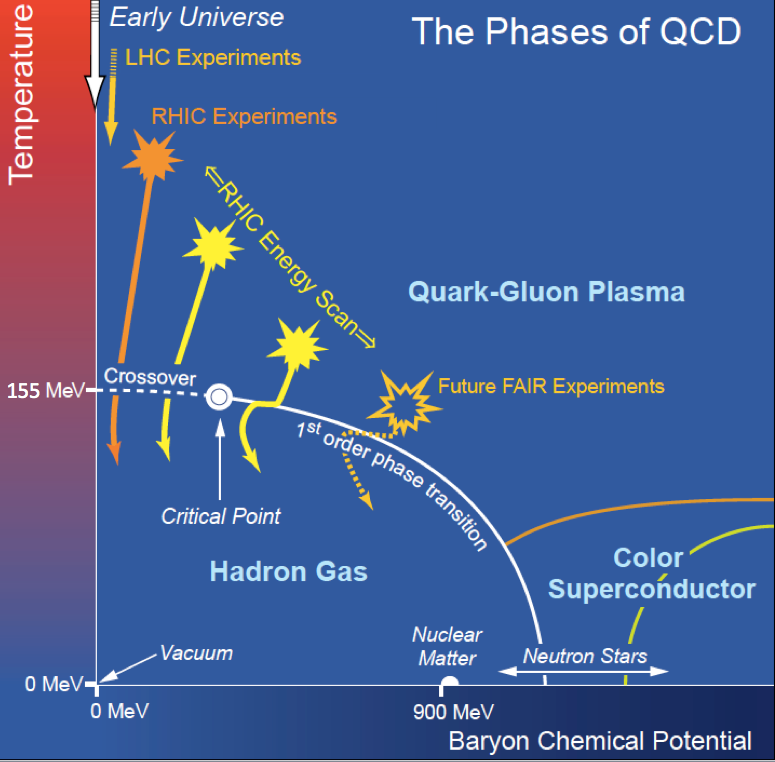
\includegraphics[width=0.65\textwidth]{fig/Phasediagram.png}}
\caption[The QCD phase diagram]{A sketch illustrating the experimental and theoretical
  exploration of the QCD phase diagram. Although experiments at
  highest energies and smallest baryon chemical potential are known to
  change from a QGP phase to a hadron gas phase through a smooth
  crossover, lower energy collisions can access higher baryon chemical
  potentials where a first order phase transition line is thought to
  exist.}
\label{F-PD1}
\end{center}
\end{figure}
%%%%%%%%%%%%%%%%%%%%% Figure PD-1 %%%%%%%%%%%%%%%%%%%%%%%%%%%%%%%%%%%%%%%%%%%%%%%
%\begin{figure}[htb]
%\begin{center}
%\begin{minipage}{0.6\textwidth}
%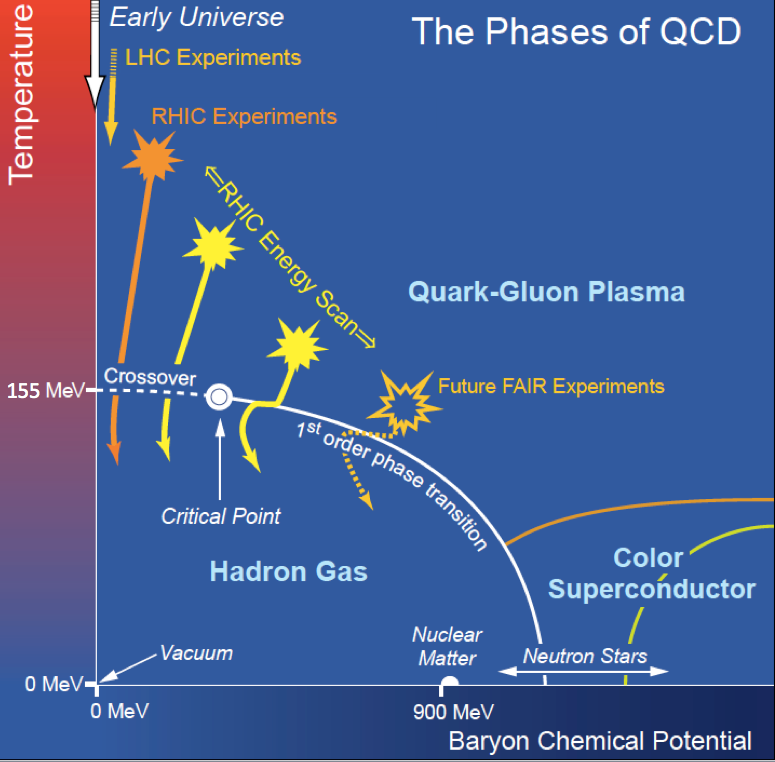
\includegraphics[width=\textwidth]{fig/Phasediagram.png}
%\end{minipage}
%\hspace*{4mm}
%\begin{minipage}{0.35\textwidth}
%\caption{A sketch illustrating the experimental and theoretical
%  exploration of the QCD phase diagram. Although experiments at
%  highest energies and smallest baryon chemical potential are known to
%  cross from a QGP phase to a hadron gas phase through a smooth
%  crossover, lower energy collisions can access higher baryon chemical
%  potentials where a first order phase transition line is thought to
%  exist.
%\label{F-PD1}
%}
%\end{minipage}
%\end{center}
%\end{figure}
%%%%%%%%%%%%%%%%%%%%%%%%%%%%%%%%%%%%%%%%%%%%%%%%%%%%%%%%%%%%%%%%%%%%%%%%%%%
%
In contrast, quark-gluon plasma doped with a sufficient excess of
quarks over anti-quarks may instead experience a sharp first order
phase transition as it cools, with bubbles of quark-gluon plasma and
bubbles of hadrons coexisting at a well-defined critical temperature,
much as bubbles of steam and liquid water coexist in a boiling
pot. The point where the doping of matter over antimatter
(parametrized by the net baryon number chemical potential $\mu_B$)
becomes large enough to instigate a first order phase transition is
referred to as the QCD critical point. It is not yet known whether QCD
has a critical point~\cite{Stephanov:1998dy,Fodor:2004nz,Allton:2005gk,Gavai:2008zr,deForcrand:2008zi},
nor where in its phase diagram it might lie. Lattice calculations
become more difficult or more indirect or both with increasing $\mu_B$
and, although new methods introduced within the past decade have
provided some hints~\cite{Fodor:2004nz,Gavai:2008zr,Datta:2012pj}.
While these theoretical calculations are advancing through both
new techniques and advances in computational power,
at present only experimental measurements can answer these questions
definitively. 


The phase diagram of QCD, with our current knowledge shown schematically
in Figure~\ref{F-PD1}, is the only phase diagram of any form of
matter in Nature that we have the opportunity of both mapping experimentally
and relating directly and quantitatively to our fundamental
description of Nature, the Standard Model. With QCD the only strongly
interacting theory in the Standard Model, mapping the transition
region of its phase diagram is a scientific goal of the highest
order. In the long term, successfully connecting a quantitative,
empirical understanding of its phases and the transitions between
phases to theoretical predictions obtained from the QCD Lagrangian
could have ramifications in how we understand phases of strongly
coupled matter in many other contexts.

%%%%%%%%%%%%%%%%%%%%%%%%%%%%%%%%%
{\bf RHIC's unique capability to probe the QCD phase diagram}
%%%%%%%%%%%%%%%%%%%%%%%%%%%%%%%%%

A major effort to use heavy ion collisions at RHIC to survey the phase
diagram of QCD is now underway. The excess of matter over antimatter
in the exploding droplet produced in a heavy ion collision can be
increased by decreasing the collision energy, which reduces the
production of matter-antimatter symmetric quark-antiquark pairs and
gluons relative to the quarks brought in by the colliding nuclei, thus
increasing $\mu_B$. Decreasing the collision energy also decreases the
maximum, {\it i.e.}~initial, temperature reached by the matter produced in
the collision. A series of heavy ion collision measurements scanning
the collision energy~\cite{BESII} can therefore explore the properties
of matter in the crossover region of the phase diagram, matter that is
neither quark-gluon plasma nor hadronic nor both at the same time, as a
function of the doping $\mu_B$. Such a program can scan the transition
region of the QCD phase diagram out to $\mu_B$ values that correspond
to collision energies below which the initial temperature no longer
reaches the transition. If the crossover region narrows to a critical
point within this experimentally accessible domain, an energy scan can
find it. RHIC completed the first phase of such an energy scan in
2014, taking data at a series of energies ($\sqrt{s_{NN}}=$ 200, 62.4,
39, 27, 19.6, 14.5, 11.5 and 7.7 GeV) corresponding to values of
$\mu_B$ that range from 20 to 400 MeV. Data from these experiments at
RHIC~\cite{Kumar:2012fb,BESII} and from previous experiments confirm that
lower-energy collisions produce matter with higher $\mu_B$, as
anticipated. 

RHIC is, and will remain, the optimal facility in the world for
mapping the phase diagram of QCD, including searching for a possible
critical point in its so far less well understood regions with larger $\mu_B$.
%studying matter in the crossover region and searching for a possible
%critical point in the so far less well understood regions of the phase
%diagram with larger $\mu_B$. 
What makes RHIC unique is both its wide
reach in $\mu_B$ and that it is a collider, meaning that the
acceptance of detectors, and hence the systematics of making
measurements, change little as a function of collision
energy. Accelerator and detector performance has been outstanding
during the first phase of this program, referred to as Beam Energy
Scan I or BES-I. Measurements of all the important observables
targeted in the planning of this campaign have now been made in
collisions with energies varying by a factor of 25, allowing for a
first look at a large region of the phase diagram of QCD.

A selection of measurements of several observables from BES-I that exhibit interesting 
non-monotonic behavior as a function of collision energy is shown in 
Section~\ref{Sec:CP}, see Figure~\ref{F-PD2} there.  
As we will discuss in that later section, the BES-I measurements of these 
observables provide some
evidence for the softening of the equation of state in the 
crossover region of the phase diagram. 
In addition, these data may indicate
the first hints of the presence of a critical point in the phase
diagram of QCD. Above all, given the size of the present
experimental uncertainties these current measurements 
provide strong motivation
for the next phase of the BES program BES-II, described in Section~\ref{Sec:CP}, which will deliver in 2018-19
substantially greater statistics and hence substantially smaller error bars
in collisions with energies at and below $\sqrt{s_{NN}}$=19.6 GeV.
Accordingly, we defer our presentation of  highlights from the rich BES-I data set to 
Section~\ref{Sec:CP}
where we will discuss each observable in a way that synthesizes
what we have learned from data to date with what can be learned
from their measurement in BES-II in combination with anticipated advances
in theory.



